\documentclass[aspectratio=169]{beamer}
\usepackage[utf8]{inputenc}
\usepackage[T1]{fontenc}
\usepackage[brazil]{babel}
\usepackage{ragged2e}
\usepackage{booktabs}
\usepackage{verbatim}
\usetheme{AnnArbor}
\usecolortheme{orchid}
\usefonttheme[onlymath]{serif}
\usepackage{listings}

\lstset{language=C,
	backgroundcolor=\color{green!10},
	basicstyle=\ttfamily,
	keywordstyle=\color{blue}\ttfamily,
	stringstyle=\color{red}\ttfamily,
	commentstyle=\color{green}\ttfamily,
	morecomment=[l][\color{magenta}]{\#}
}

\AtBeginSection[]{
  \begin{frame}
  \vfill
  \centering
  \begin{beamercolorbox}[sep=8pt,center,shadow=true,rounded=true]{title}
    \usebeamerfont{title}\insertsectionhead\par%
  \end{beamercolorbox}
  \vfill
  \end{frame}
}

\title[\sc{Recursão}]{Recursão}
\author[Roland Teodorowitsch]{Roland Teodorowitsch}
\institute[ALEST I - EP - PUCRS]{Algoritmos e Estruturas de Dados I - Escola Politécnica - PUCRS}
\date{10 de agosto de 2023}

\begin{document}
\justifying

%-------------------------------------------------------
\begin{frame}
	\titlepage
\end{frame}

%=======================================================
\section{Recursão}

%-------------------------------------------------------
\begin{frame}\frametitle{Leitura(s) Recomendada(s)}

\begin{columns}[T]
\begin{column}{0.15\linewidth}
\vspace{-3mm}
\begin{figure}[h]
	\centering
	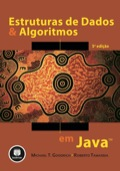
\includegraphics[height=0.3\paperheight]{imagens/livro_goodrich.jpg}
\end{figure}
\end{column}
\begin{column}{0.85\linewidth}
\vspace{3mm}
\textbf{Seção 3.5}\\
\scriptsize{GOODRICH, Michael T.; TAMASSIA, Roberto. \textbf{Estruturas de dados e algoritmos em Java}. Tradução: Bernardo Copstein. 5. ed. Porto Alegre: Bookman, 2013. xxii, 713 p. E-book. ISBN 9788582600191. Tradução de: Data Structures and Algorithms in Java, 5th Edition. Disponível em: \textless{}\url{https://integrada.minhabiblioteca.com.br/\#/books/9788582600191/}\textgreater{}. Acesso em: 01 ago. 2023.}
\end{column}
\end{columns}

\end{frame}

%-------------------------------------------------------
\begin{frame}\frametitle{Algoritmo recursivo}
\begin{itemize}
	\item É um algoritmo que faz chamada a si próprio dentro de sua implementação
	\item \textbf{Importante:} o algoritmo deve garantir que a recursão termine
	\begin{itemize}
		\item Do contrário se entrará em um laço infinito
		\item Importante considerar a condição de termino logo no início da implementação do algoritmo
	\end{itemize}
\end{itemize}
\end{frame}

%-------------------------------------------------------
\begin{frame}\frametitle{Exemplo clássico: fatorial}
\begin{itemize}
	\item O fatorial de n é normalmente definido como:
\[ n! = \prod_{k=1}^{n}{k} = n \times (n-1) \times (n-2) \times ... \times 3 \times 2 \times 1,\qquad \forall n \in \mathbb{N}\]
	\item Por exemplo:
\[5 ! = 5 \times 4 \times 3 \times 2 \times 1 = 120\]
	\item Mas também pode-se usar a sua definição recursiva:
\[ n! = \begin{cases}
1, & \mbox{se ~ } n=0 \mbox{~ ou ~ } n=1\\
n \times (n-1)!, & \mbox{se ~ } n > 1
\end{cases} \]
\end{itemize}
\end{frame}

%-------------------------------------------------------
\begin{frame}[fragile]\frametitle{Implementação do fatorial}
\begin{itemize}
	\item Iterativo
{\scriptsize\lstinputlisting{src/fatorial.c}}
	\item Recursivo
{\scriptsize\lstinputlisting{src/fatorialRec.c}}
	\end{itemize}
\end{frame}

%-------------------------------------------------------
\begin{frame}\frametitle{Rastreamento Recursivo}
\begin{figure}[h]
	\centering
	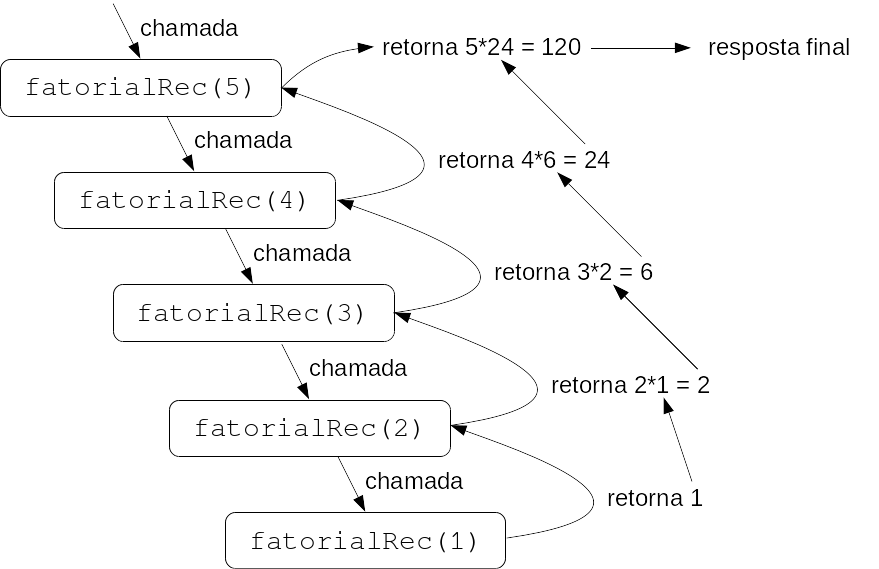
\includegraphics[height=0.7\paperheight]{imagens/rastreamento_recursivo.png}
\end{figure}
\end{frame}

%-------------------------------------------------------
\begin{frame}\frametitle{Recursividade}
\begin{itemize}
	\item Poderosa ferramenta de programação
	\item Apesar de bastante empregada, nem sempre ela deve ser aplicada
	\begin{itemize}
		\item É preciso analisar o problema e ver se necessita de uma solução recursiva
	\end{itemize}
	\item Quando bem empregada pode tornar a solução de um problema clara, simples e consisa
\end{itemize}
\end{frame}

%-------------------------------------------------------
\begin{frame}\frametitle{...}
\begin{itemize}
	\item ...	
\end{itemize}
\end{frame}

%-------------------------------------------------------
\begin{frame}\frametitle{Vantagens}
\begin{itemize}
	\item Rotinas mais concisas
	\item Relação direta com uma prova por indução matemática
	\begin{itemize}
		\item Indução matemática: metodo de prova matemática usado para demonstrar a verdade de um número infinito de proposições
		\begin{itemize}
			\item Válida se funciona para $n$ igual a $0$ ou $1$
			\item Válida se vale para $n$ igual a $k$ e $k + 1$
		\end{itemize}
		\item Facilita verificar a correção
	\end{itemize}
\end{itemize}
\end{frame}

%-------------------------------------------------------
\begin{frame}\frametitle{Desvantagens}
\begin{itemize}
	\item Cada chamada recursiva implica em um custo (tempo e espaço)
	\begin{itemize}
		\item Informações são armazenadas na pilha
		\item Para cada chamada realizada, um conjunto de variáveis locais é alocado (criado)
		\item Cada chamada requer
		\begin{itemize}
			\item O empilhamento de parâmetros e endereços de retorno da função que chama
			\item O desempilhamento de parâmetros pela função que executa
		\end{itemize}
		\item Cada retorno requer
		\begin{itemize}
			\item O desempilhamento do endereço de retorno
			\item O empilhamento do resultado (ou passagem por registrador)
			\item O desempilhamento do retorno pela função que chamou
		\end{itemize}
	\end{itemize}
\end{itemize}
\end{frame}

%-------------------------------------------------------
\begin{frame}\frametitle{Exercícios}
\begin{enumerate}
	\item Faça o algoritmo da potência de forma não recursiva e de forma recursiva. Considere que o valor da base e do expoente são recebidos por parâmetro, inteiros e positivos.
	\item Faça um algoritmo recursivo que inverta a ordem dos elementos de um vetor.
	\item Faça um algoritmo recursivo para somar os elementos de um vetor.
	\item \textbf{Desafio:}\\
	Faça um algoritmo recursivo para verificar se uma cadeia de caracteres é um palíndromo.\\
	Teste: ``socorrammesubinoonibusemmarrocos''.
\end{enumerate}
\end{frame}

%=======================================================
\section{Créditos}

%-------------------------------------------------------
\begin{frame}\frametitle{Créditos}
\begin{itemize}
	\item Estas lâminas contêm trechos de materiais criados e disponibilizados pelo professor Iaçanã Ianiski Weber.
\end{itemize}
\end{frame}

%-------------------------------------------------------
\end{document}

